\subsection{Newton’s Fluxions: From Geometry to Motion (1670s)}

Building on the geometric insights of his teacher Barrow, Isaac Newton carried the idea of infinitesimal change to its logical extreme. While Barrow had described the relation between curves and their tangents through proportions, Newton reframed the entire question in terms of \textit{motion}.

To Newton, quantities were not static magnitudes, but flowing values—changing continuously with time. Instead of drawing triangles on curves, he imagined how a point moved along a curve, and how its position evolved. This shift—from shape to speed, from geometry to kinematics—transformed the mathematics of the curve into the mathematics of change itself.

Where Barrow described a tangent as the limit of geometric constructions, Newton described it as the result of a process: the \textit{fluxion} of a quantity, or its instantaneous rate of change.

\vspace{1em}

He denoted this with a dot over the variable:

\[
\dot{x} = \frac{o}{\bar{o}}
\]

where:

\begin{itemize}
    \item \( o \) is an \textbf{infinitely small increment} of time.  
    \item \( \bar{o} \) is the corresponding change in \( x \).
\end{itemize}

Unlike his predecessors, Newton did not merely approximate motion—he embedded it into the foundations of his system. Tangents were no longer assumptions, nor constructions: they were consequences of how quantities flowed.

\vspace{0.5em}

\textit{Where Cavalieri stacked indivisibles, and Barrow drew proportional curves, Newton let quantities move—and built calculus on their motion.}


\begin{figure}[H]
\centering
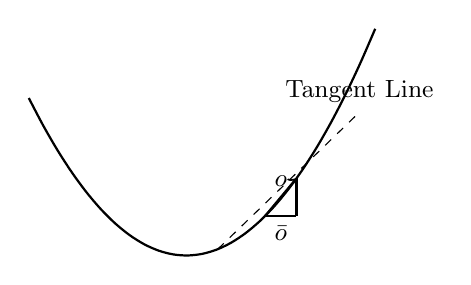
\begin{tikzpicture}[scale=2]
    % Draw the curve
    \draw[thick, domain=-1:1.2, smooth, variable=\x] plot ({\x},{\x*\x});

    % Draw infinitesimal motion
    \draw[->, thick] (0.5, 0.25) -- (0.7, 0.49) node[midway, above] {\small $o$};
    \draw[thick] (0.5, 0.25) -- (0.7, 0.25);
    \draw[thick] (0.7, 0.25) -- (0.7, 0.49);
    \node[below] at (0.6,0.25) {\small $\bar{o}$};
    
    % Draw tangent line
    \draw[dashed] (0.2, 0.04) -- (1.1, 0.91) node[above] {\small Tangent Line};

\end{tikzpicture}

\vspace{0.5em}
\caption{\small Newton's conception of calculus was rooted in geometry and motion. He imagined a point moving along a curve, where the instantaneous rate of change — the fluxion — could be represented as the ratio between an infinitesimal vertical change ($o$) and an infinitesimal horizontal change ($\bar{o}$). The resulting quantity corresponds to the slope of the tangent line at that point. This approach reflects Newton’s view of change as inherently tied to physical movement through time.}
\end{figure}

